\section{特殊成员函数的规则}
让我们来讨论一下特殊成员函数,特别是确切地指定何时以及如何生成特殊的复制和移动成员函数。

\subsection{特殊的成员函数}

首先简单地看看特殊成员函数,因为它以不同的方式使用。C++标准将以下6种操作定义为特殊成员函数:

\begin{itemize}
	\item 默认构造函数
	\item 复制构造函数
	\item 复制赋值运算符
	\item 移动构造函数(C++11)
	\item 移动赋值操作符(C++11)
	\item 析构函数
\end{itemize}

然而,在许多情况下,我们只讨论其中5个操作,因为默认构造函数与其他5个(或C++11之前的3个)操作略有不同。其他5个操作通常没有声明,并且具有更复杂的依赖关系。因此,请了解特殊成员函数的含义(到目前为止,我一直试图避免使用这个术语)。

图3.1概述了什么时候会根据声明的构造函数和特殊成员函数,自动生成特殊成员函数:

\begin{picture}
	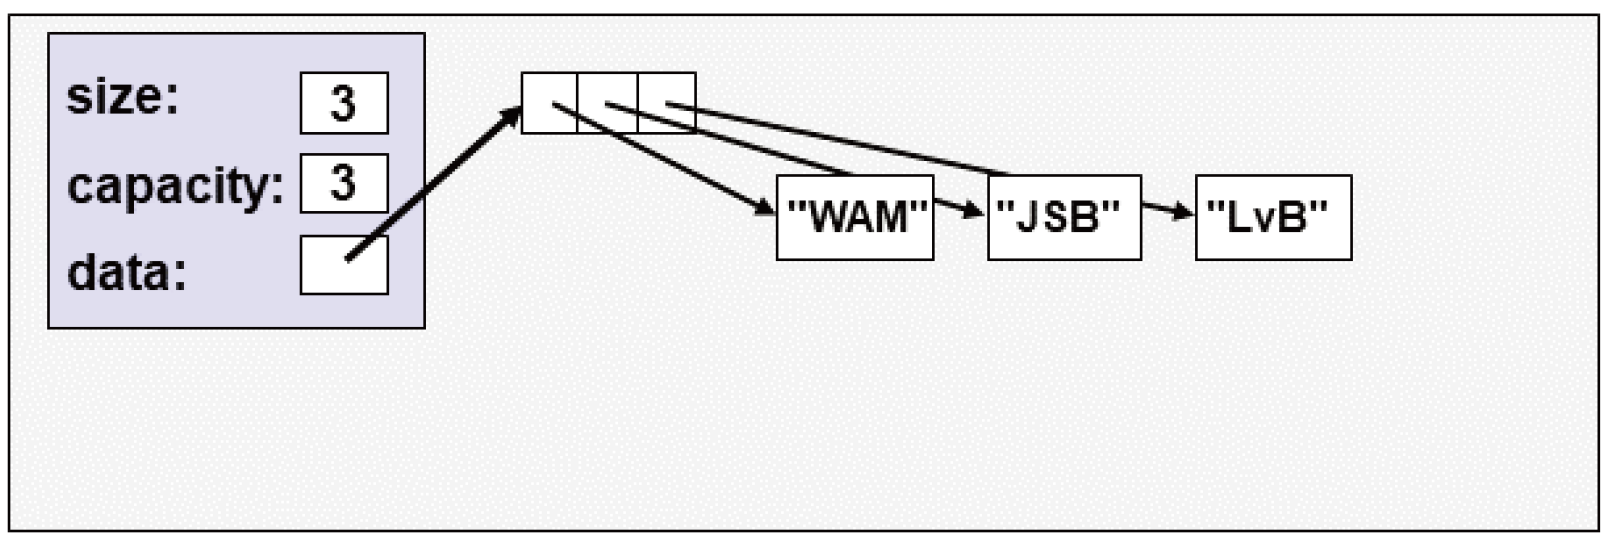
\includegraphics[width=1.0\textwidth]{content/1/chapter3/images/1}
	\caption{自动生成特殊成员函数的规则}
\end{picture}


可以在这个表格中看到一些基本的规则:

\begin{itemize}
	\item 只有在没有用户声明其他构造函数的情况下,才会自动声明默认构造函数。
	\item 特殊的复制成员函数和析构函数禁用了移动支持。自动生成特殊的移动成员函数是禁用的(除非也声明了移动操作)。但是,移动对象的请求通常是有效的,因为复制成员函数用作后备(除非特殊的移动成员函数显式删除)。
	\item 特殊的移动成员函数禁用了正常的复制和赋值。复制和其他移动特殊成员函数将删除,这样只能移动(分配)对象,而不能复制(分配)对象(除非还声明了其他操作)。
\end{itemize}

\subsection{默认情况下,有复制和移动}

在默认编译情况下,为类生成复制和移动特殊成员函数。

假设类\textit{Person}的声明如下:

\begin{cppcode}
class Person {
	...
public:
	...
	// NO copy constructor/assignment declared
	
	// NO move constructor/assignment declared
	
	// NO destructor declared
};
\end{cppcode}

这种情况下,\textit{Person}可以复制和移动:

\begin{cppcode}
std::vector<Person> coll;

Person p{"Tina", "Fox"};
coll.push_back(p); // OK, copies p
coll.push_back(std::move(p)); // OK, moves p
\end{cppcode}

\subsection{已声明的复制禁用移动(启用退阶)}

在声明复制特殊成员函数(或析构函数)时,禁用了移动特殊成员函数的自动生成:

假设\textit{Person}的声明如下:

\begin{cppcode}
class Person {
	...
public:
	...
	// copy constructor/assignment declared:
	Person(const Person&) = default;
	Person& operator=(const Person&) = default;
	
	// NO move constructor/assignment declared
};
\end{cppcode}

因为退阶机制是有效的,所以复制和移动\textit{Person}可以编译,但移动是作为复制执行的:

\begin{cppcode}
std::vector<Person> coll;

Person p{"Tina", "Fox"};
coll.push_back(p); // OK, copies p
coll.push_back(std::move(p)); // OK, copies p
\end{cppcode}

因此,用\textit{=default}声明一个特殊成员函数与根本不声明它是不同的。复制构造函数和复制赋值操作符是用户声明的,它禁用了移动构造和移动赋值,以便移动到副本。声明的析构函数具有相同的效果。

您可能想知道为什么声明的析构函数会禁用移动语义。关于已移动状态那一章讨论了具体的例子,一个类的析构函数导致生成的移动语义不能正常工作。

\subsection{声明移动,禁用复制}

如果声明了的移动语义,就禁用了复制语义。删除复制特殊成员函数。

换句话说,如果移动构造函数或移动赋值操作符显式声明(使用\textit{=default}实现、生成,或使用\textit{=delete}禁用),那么通过使用\textit{=delete}声明,就禁用了调用复制构造函数和复制赋值操作符。

假设\textit{Person}的声明如下:

\begin{cppcode}
class Person {
	...
	public:
	...
	// NO copy constructor declared
	
	// move constructor/assignment declared:
	Person(Person&&) = default;
	Person& operator=(Person&&) = default;
};
\end{cppcode}

本例中,我们有一个只移动类型。Person可以移动,但不能复制:

\begin{cppcode}
std::vector<Person> coll;

Person p{"Tina", "Fox"};
coll.push_back(p); // ERROR: copying disabled
coll.push_back(std::move(p)); // OK, moves p

coll.push_back(Person{"Ben", "Cook"}); // OK, moves temporary person into coll
\end{cppcode}

同样,使用\textit{=default}声明特殊成员函数与根本不声明不同。调用的后果更加严重:复制对象的尝试将无法编译。

支持移动操作但不支持复制操作的类是有意义的。可以使用这种只移动类型传递资源的所有权或句柄,而无需共享或复制。在C++标准库中也有一些只移动的类型(例如,输入输出流、线程和\textit{std::unique_ptr<>}),详细信息请参见关于仅移动类型的章节。

\subsection{删除移动没有意义}

出于同样的原因,如果将移动构造函数声明为\textit{delete},则不能移动(已禁用此操作,没有使用任何退阶)和不能复制(因为声明的移动构造函数禁用了复制操作):

\begin{cppcode}
class Person {
public:
	...
	// NO copy constructor declared
	// move constructor/assignment declared as deleted:
	Person(Person&&) = delete;
	Person& operator=(Person&&) = delete;
	...
};

Person p{"Tina", "Fox"};
coll.push_back(p); // ERROR: copying disabled
coll.push_back(std::move(p)); // ERROR: moving disabled
\end{cppcode}

通过声明复制被删除的特殊成员函数,可以获得相同的效果,这可能不会让其他程序员感到困惑。

删除移动操作和启用复制操作真的没有意义:

\begin{cppcode}
class Person {
	public:
	...
	// copy constructor explicitly declared:
	Person(const Person& p) = default;
	Person& operator=(const Person&) = default;
	
	// move constructor/assignment declared as deleted:
	Person(Person&&) = delete;
	Person& operator=(Person&&) = delete;
	...
};

Person p{"Tina", "Fox"};
coll.push_back(p); // OK: copying enabled
coll.push_back(std::move(p)); // ERROR: moving disabled
\end{cppcode}

这种情况下,\textit{=delete}禁用了退阶机制(因此也与根本不声明它不同)。编译器找到该声明并报告该调用为错误。

支持复制但在调用移动时失败的类型没有任何意义。对于此类的用户,复制有时可行,有时不行。作为指导原则:永不\textit{=delete}特殊的移动成员函数。如果想要同时禁用复制和移动,删除复制的特殊成员函数就足够了。

\subsection{禁用移动语义与启用复制语义}

基于我们刚才讨论的内容,现在知道了当复制仍然有意义时如何禁用移动语义。将特殊的移动成员函数声明为已删除通常不是正确的做法,因为它禁用了退阶机制。

提供复制语义的同时,禁用移动语义的正确方法是,声明另一个特殊成员函数(复制构造函数、赋值操作符或析构函数)。我建议你使用默认复制构造函数和赋值操作符(声明其中一个就足够了,但可能会造成不必要的混淆):

\begin{cppcode}
class Customer {
	...
public:
	...
	Customer(const Customer&) = default; // disable move semantics
	Customer& operator=(const Customer&) = default; // disable move semantics
};
\end{cppcode}

因为没有发现生成的特殊的移动成员函数,所以现在会复制临时的\textit{Customer},甚至标记为\textit{std::move()}的\textit{Customer}对象:

\begin{cppcode}
std::vector<Customer> customers;
...
customers.push_back(createCustomer()); // OK, falls back to copying
customers.push_back(std::move(customers[0])); // OK, falls back to copying
\end{cppcode}

但是,通常最好是实现特殊的移动成员函数,来修复默认生成的移动操作所存在的任何问题。关于迁移状态的章节将讨论实践中的例子。

请注意,只有声明特殊的复制成员函数才会违反“5规则”,我们将在后面详细讨论这个规则。必须声明特殊的复制成员函数,但也不能声明特殊的移动成员函数(删除和默认都不能工作,实现它们会使类变得复杂)。因此,如果显式地声明一个复制特殊成员函数只是为了禁用移动语义,请添加一个注释,以确保该声明不会被特殊移动成员函数的声明删除或扩展。

\subsection{为禁用移动语义的成员进行移动}

如果某个类型的移动语义不可用或已被删除,则这不会影响具有此类型成员的类的移动语义的生成。生成的默认移动构造函数和赋值操作符逐个成员决定是复制还是移动它。如果移动不可能(即使移动操作被删除),则生成一个副本(如果可能的话)。

例如,以下类:

\begin{cppcode}
class Customer {
	...
public:
	...
	Customer(const Customer&) = default; // copying calls enabled
	Customer& operator=(const Customer&) = default; // copying calls enabled
	Customer(Customer&&) = delete; // moving calls disabled
	Customer& operator=(Customer&&) = delete; // moving calls disabled
};
\end{cppcode}

如果这个类被另一个类中的成员使用:

\begin{cppcode}
class Invoice {
	std::string id;
	Customer cust;
public:
	... // no special member functions
};
\end{cppcode}

生成的移动构造函数将移动\textit{id}字符串,但复制客户的\textit{cust}:

\begin{cppcode}
Invoice i;
Invoice i1{std::move(i)}; // OK, moves id, copies cust
\end{cppcode}

\subsection{生成的特殊成员函数的规则}

现在我们可以总结特殊成员函数的新规则(何时生成它们以及它们的行为方式)。

例如,假设有以下派生类:

\begin{cppcode}
class MyClass : public Base
{
private:
	MyType value;
	...
};
\end{cppcode}

这里缺少noexcept,我们将在后面关于noexcept的章节中介绍它,但我们会在这里提到相应的保证。

\subsubsection{复制构造函数}

当应用以下所有内容时,将自动生成复制构造函数:

\begin{itemize}
	\item 用户没有声明移动构造函数
	\item 用户没有声明移动赋值操作符
\end{itemize}

如果生成(隐式或使用\textit{=default}),复制构造函数具有以下行为:

\begin{cppcode}
MyClass(const MyClass& obj) noexcept-specifier
: Base(obj), value(obj.value) {
}
\end{cppcode}

生成的复制构造函数,首先将源对象传递给基类的最佳匹配的复制构造函数。(记住,复制构造函数总是在自顶向下的基础上调用)。它倾向于使用具有相同声明的复制构造函数(通常声明为\textit{const\&})。如果不可用,可能会调用下一个最佳匹配的构造函数(例如,复制构造函数模板)。然后,复制类的所有成员(同样使用最佳匹配)。

生成的复制构造函数声明为noexcept,除非所有复制操作(所有基类的复制构造函数和所有成员的复制构造函数)都有这个保证。

\subsubsection{移动构造函数}

移动构造函数在应用以下所有条件时自动生成:

\begin{itemize}
	\item 用户没有声明复制构造函数
	\item 用户没有声明复制赋值操作符
	\item 用户没有声明移动赋值操作符
	\item 用户没有声明析构函数
\end{itemize}

如果生成(隐式或使用\textit{=default}),移动构造函数具有以下行为:

\begin{cppcode}
MyClass(MyClass&& obj) noexcept-specifier
: Base(std::move(obj)), value(std::move(obj.value)) {
}
\end{cppcode}

生成的移动构造函数首先传递源对象(标记为\textit{std::move()}来传递移动语义),给基类最佳匹配的移动构造函数。最佳匹配的移动构造函数通常是具有相同声明(用\&\&声明)的构造函数。然而,如果这是不可用的,可能会调用下一个最佳匹配的构造函数(例如,移动构造函数模板,甚至复制构造函数)。然后,移动类的所有成员(同样使用最佳匹配)。

生成的移动构造函数声明为noexcept,除非所有调用的移动/复制操作(所有基类的复制或移动构造函数,以及所有成员的复制或移动构造函数)都保证了这一点。

\subsubsection{复制赋值运算符}

复制赋值操作符在应用以下所有条件时自动生成:

\begin{itemize}
	\item 用户没有声明移动构造函数
	\item 用户没有声明移动赋值操作符
\end{itemize}

如果生成(隐式或使用\textit{=default}),复制赋值操作符大致具有以下行为:

\begin{cppcode}
MyClass& operator= (const MyClass& obj) noexcept-specifier {
	Base::operator=(obj); // - perform assignments for base class members
	value = obj.value; // - assign new members
	return *this;
}
\end{cppcode}

生成的复制赋值操作符,首先对传递的源对象调用基类的最佳匹配赋值操作符(记住,与复制构造函数相比,赋值操作符不是自上而下调用的;它们在实现中调用基类赋值操作符)。然后,为其类的成员进行分配(同样使用最佳匹配)。

注意,生成的赋值操作符不会检查对象对自赋值。如果这很重要,必须自己实现操作符。

此外,生成的复制赋值操作符声明为noexcept,除非所有赋值操作(基类成员的赋值和新成员的赋值)都给出了这个保证。

\subsubsection{移动赋值操作符}

移动赋值操作符在以下所有条件都适用时自动生成:

\begin{itemize}
	\item 用户没有声明复制构造函数
	\item 用户没有声明移动构造函数
	\item 用户没有声明复制赋值操作符
	\item 用户没有声明析构函数
\end{itemize}

如果生成(隐式或使用\textit{=default}),移动赋值操作符大致具有以下行为:

\begin{cppcode}
MyClass& operator= (MyClass&& obj) noexcept-specifier {
	Base::operator=(std::move(obj)); // - perform move assignments for base class members
	value = std::move(obj.value); // - move assign new members
	return *this;
}
\end{cppcode}

生成的移动赋值操作符,首先为传递的源对象调用基类的最佳匹配的移动赋值操作符,用\textit{std::move()}标记来传递移动语义。然后它移动分配它的类的所有成员(同样使用最佳匹配)。

你可能想知道,为什么在源对象标记为\textit{std::move()}之后,我们仍然使用对象obj的成员:

\begin{cppcode}
Base::operator=(std::move(obj)); // - perform move assignments for base class members
\end{cppcode}

本例中,将对象标记为基类的特定上下文,基类不能看到在该类中引入的成员。因此,派生成员具有有效但未定义的状态,但仍然可以使用新成员的值。

生成的赋值操作符也不会检查对象对自赋值。因此,在默认行为中,操作符将把每个成员都赋值给自身,这通常意味着成员接收一个有效但未定义的值。如果这很重要,需要自己实现操作符。

此外,生成的移动赋值操作符被声明为noexcept,除非所有调用的赋值操作(基类成员的赋值和新成员的赋值)都保证了这一点。

\subsubsection{其他特殊成员函数}

其他特殊成员函数对移动语义没有那么重要的作用:

\begin{itemize}
	\item 析构函数对于移动语义没有什么特别之处,除了声明禁用了移动操作的自动生成。
	\item 如果没有声明其他构造函数,默认构造函数(“不那么特殊”的特殊成员函数)仍然会自动生成。也就是说,移动构造函数的声明禁用了默认构造函数的生成。
\end{itemize}

但请注意,当谈到已移动状态时,这些特殊的成员函数发挥了作用。默认构造函数的状态通常是已移动对象的“自然”状态,而已移动对象是可销毁的。
















